%! Author = chaorn
%! Date = 13.08.24

\subsection{Fuzzing mit AFLNet}\label{subsec:aflnet}
Das folgende Kapitel beschreibt das Aufsetzen der Testumgebung und die darin durchgeführten Experimente mit dem Fuzzing-Tool
\gls{afl}Net.
\subsubsection{Setup}
Da \gls{afl}Net legacy Software ist, wird es nicht mehr aktiv weiterentwickelt und an neue Frameworks und Bibliotheken
angepasst.
Zum Kompilieren von \gls{afl}Net wird hierzu ein angepasstes Dockerfile~\cite{aflnet-dockerfile} verwendet.
Dieses angepasste Dockerfile enthält alle notwendigen Abhängigkeiten, um \gls{afl}Net zu kompilieren.
Hierzu zählen die Abhängigkeiten \texttt{llvm} und \texttt{clang} in der Version 11.
\texttt{llvm} wird benötigt, um den \gls{afl} Compiler \texttt{afl-clang-fast} zu kompilieren.
Dieser wird für optimierte Instrumentierung des Codes des \gls{zup} verwendet und bezweckt somit höhere Ausführgeschwindigkeiten
während der Fuzzing Kampagne.
Für die erfolgreiche Verwendung des Compilers \texttt{afl-clang-fast} musste für die Kompatibilität mit einer neueren
Ubuntu-Version ein Patch~\cite{llvm-patch} für das Kompilieren des Compilers geschrieben werden.\newline
Das \gls{zup} Mosquitto wird ebenfalls in einem Docker Container kompiliert.
Hierzu wird der Compiler \texttt{afl-clang-fast} verwendet.
Die Instrumentierung des Codes erfolgt durch das Flag \texttt{-fsanitize=address}.
Dieses Flag aktiviert \textit{address sanitization} und ermöglicht es, dass \gls{afl}Net die Speicherzugriffe des \gls{zup}
überwachen kann und somit Buffer Overflows und Memory Leaks erkennt.
Zum Starten des Mosquitto-Bianrys wurde außerdem eine \textit{preloaded-library}~\cite{mqtt-preload} verwendet, die alle Ausgaben des \gls{zup}
aus den Kanälen \texttt{stdout} und \texttt{stderr} in eine log-Datei \texttt{mqtt-aflnet\_stdout.log} weiterleitet.
Diese Log-Datei wird benötigt, um die Ausgaben des \gls{zup} zu analysieren und somit die Effektivität der generierten
Testcases zu bewerten. \newline
Die Testcases wurden mithilfe eines Python-Skripts~\cite{aflnet-generate-test} generiert.
Die Struktur wurde hierzu aus bereits existierenden Nachrichten einer \gls{pcap}-Datei mithilfe von Wireshark extrahiert.
Anhand der Struktur der Bytes wurden die Nachrichten in ein Format umgewandelt, das von \gls{afl}Net verstanden wird.
Die in Kapitel~\ref{subsec:mosquitto-mqtt} beschriebene Struktur einer \gls{mqtt} Nachricht wurde dazu verwendet.
In dieser Nachricht kann der Fixed-Header den Bytes \texttt{0x10, 0x30, 0x82, 0xA2, 0xC0} und \texttt{0xE0} entsprechen.
Diese stehen für die verschiedenen Anfragen \texttt{CONNECT, PUBLISH, SUBSCRIBE, UNSUBSCRIBE, PINGREQ} und \texttt{DISCONNECT}.
Die Variable Header und Payload wurden zufällig generiert und in die Testcases eingefügt.
Die Testcases wurden in einem Verzeichnis \texttt{aflnet\_in/} abgelegt und von \gls{afl}Net als Eingabe verwendet.
Damit möglichst viele States beim Ausführen des \gls{zup} erreicht werden, wurden ebenfalls ungültige Pakete generiert.
Sie dienen \gls{afl}Net dazu, unerwartete Zustände des \gls{zup} zu erreichen und somit unerwartete Bugs zu finden.
Des Weiteren wurden Nachrichtensequenzen generiert, die den Zustand des \gls{zup} verändern.
Hierzu wurden alle Nachrichten, die der \gls{zup} verarbeiten kann, in einer Sequenz aneinandergereiht.
Diese Sequenzen wurden ebenfalls in das Verzeichnis \texttt{aflnet\_in/} abgelegt und von \gls{afl}Net als Eingabe verwendet.
\subsubsection{Analyse der Effektivität gesendeter Pakete}
Die Fuzzing-Kampagne wurde über einen Zeitraum von 48 Stunden durchgeführt.
Zur Analyse der Effektivität der gesendeten Pakete wurde eine preload bibliothek verwendet, die die Ausgaben des \gls{zup}
der Kanäle \texttt{sdtout} und \texttt{stderr} in eine Log-Datei \texttt{mqtt-aflnet\_stdout.log} umleitet.
Mit den folgenden Experimenten und Auswertungen soll ein Teil der Forschungsfrage \textit{Q1}~\ref{researc-questions}
beantwortet werden.
Nun wird analysiert, wie effektiv die generierten Nachrichten des \gls{afl}Net-Fuzzers sind.\newline
Diese Log-Datei wurde auf die Häufigkeit der Ausgaben von erfolgreichen und fehlgeschlagenen Verbindungsaufbauten analysiert.
\begin{figure}[H]
    \centering
    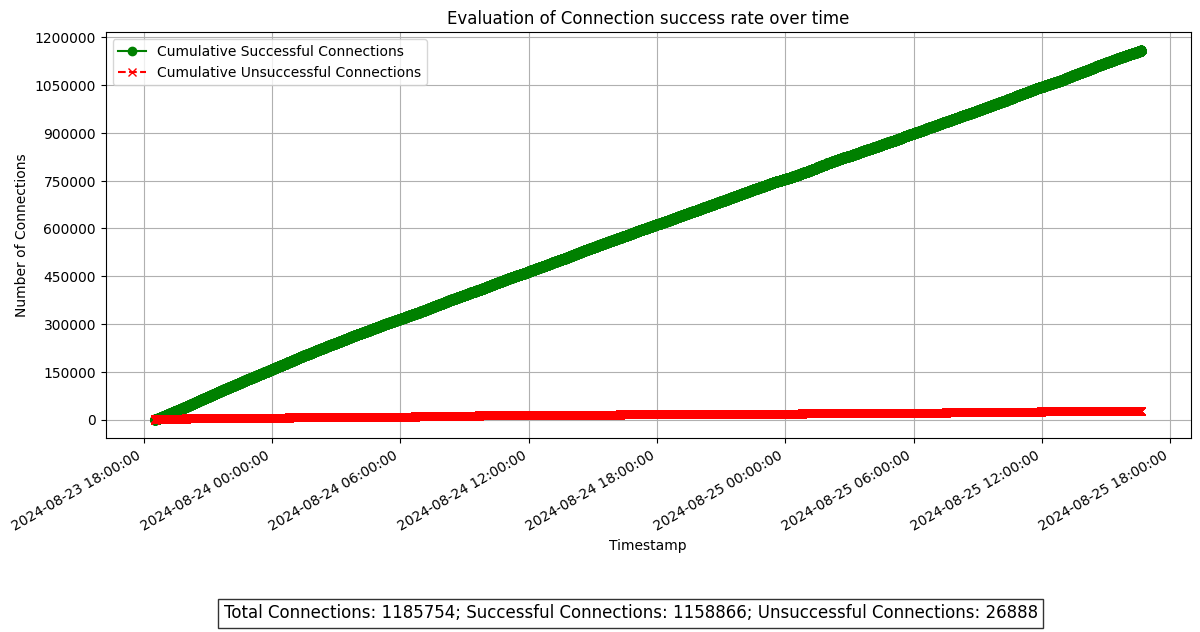
\includegraphics[width=\textwidth]{img/connection_evaluation_aflnet}
    \caption[Diagram zur Auswertung erfolgreicher Verbindungsaufbauten mit dem \gls{mqtt}-Protokoll]{Evaluation der Verbindungsaufbauten des \gls{zup} Mosquitto. Die Log-Datei \texttt{mqtt-aflnet\_stdout.log}
    wurde auf die Häufigkeit der Ausgaben von erfolgreichen und fehlgeschlagenen Verbindungsaufbauten analysiert.}
    \label{fig:mqtt-aflnet_stdout}
\end{figure}
\noindent Die grüne Linie (siehe Abb.~\ref{fig:mqtt-aflnet_stdout}) repräsentiert die Anzahl der erfolgreichen Verbindungen im Laufe der Zeit.
Die Linie steigt linear an und erreicht gegen Ende der Kampagne eine Gesamtzahl von 1.158.866 erfolgreichen Verbindungen.
Dies deutet darauf hin, dass das getestete System eine sehr hohe Erfolgsrate bei Verbindungsversuchen aufweist.
Die lineare Zunahme zeigt, dass die Rate der erfolgreichen Verbindungen konstant hoch geblieben ist, ohne signifikante
Einbrüche oder Schwankungen.
Die rote Linie (siehe Abb.~\ref{fig:mqtt-aflnet_stdout}) zeigt die Anzahl der erfolglosen Verbindungen an.
Diese bleibt über den gesamten Zeitraum sehr niedrig und erreicht gegen Ende der Kampagne etwa 26.888 erfolglose Verbindungen.
Dies entspricht einer Erfolgsrate von über \SI{97}{\percent} und einer Fehlerrate von ca. $\sim \SI{2.32}{\percent}$
in denen \gls{afl}Net keine erfolgreichen Verbindungsaufbauten mit dem \gls{mqtt}-Broker über das \gls{mqtt}-Protokoll
entstanden sind.
Der minimale Anstieg im Vergleich zu den erfolgreichen Verbindungen weist darauf hin, dass die Mehrheit der Verbindungen
erfolgreich war.
Bei der Analyse der Fehleranfälligkeit von nicht validen Nachrichten wurde festgestellt, dass am Anfang der Fuzzing-Kampagne
viele Fehlermeldungen auftraten.
Mit der Zeit wurden jedoch weniger Fehlermeldungen generiert, da die State Machine des \gls{zup} erlernt wurde und somit
vermehrt valide Nachrichten generiert wurden.
\begin{figure}[H]
    \centering
    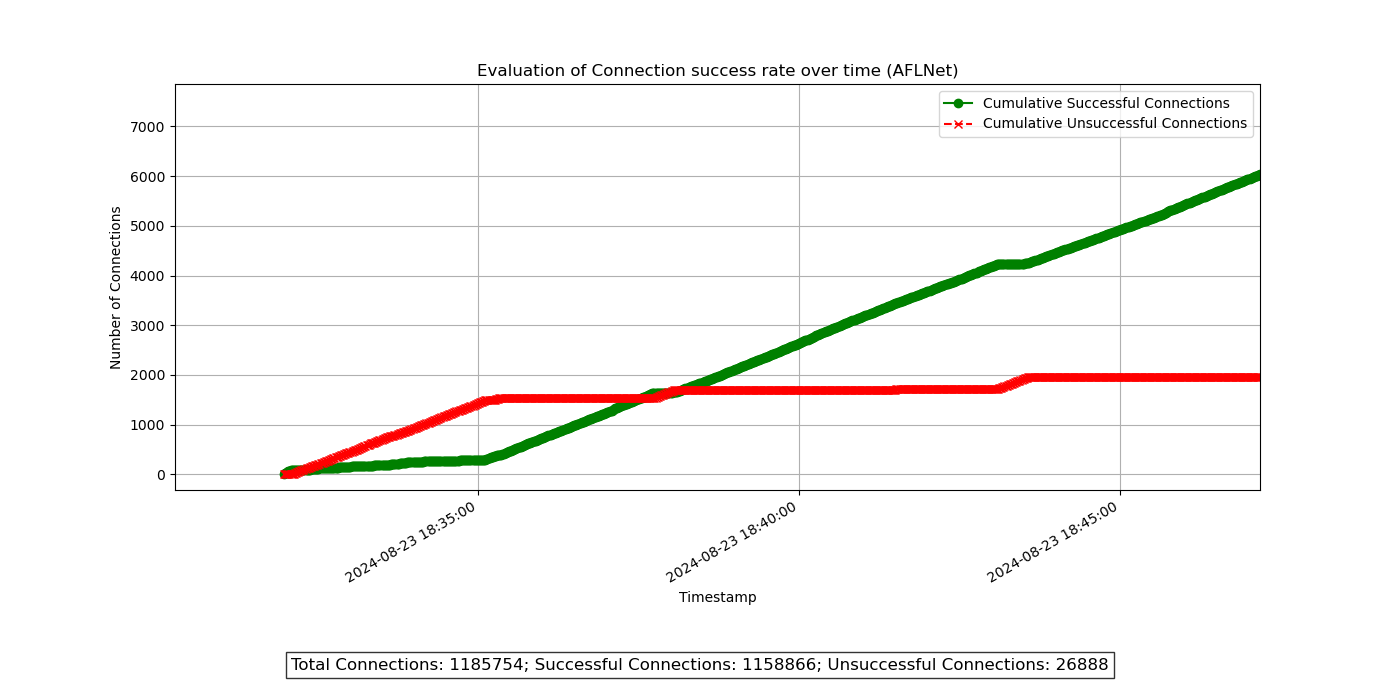
\includegraphics[width=\textwidth]{img/connection_evaluation_aflnet_beginning}
    \caption[Diagram zur Auswertung erfolgreicher Verbindungsaufbauten mit dem \gls{mqtt}-Protokoll zu Beginn der Fuzzing Kampagne]{
        Dieses Diagramm zeigt eine vergrößerte Ansicht der ersten
        10 Minuten der Fuzzing-Kampagne aus Abbildung~\ref{fig:mqtt-aflnet_stdout} mit \gls{afl}Net zur Veranschaulichung der Fehleranfälligkeit zu Beginn der Fuzzing-Kampagne.
        Aus dem Diagramm geht hervor, dass zu Beginn der Kampagne viele erfolglose Verbindungen mit dem \gls{zup} generiert
        wurden, die jedoch im Laufe der Zeit abnahmen.
    }
    \label{fig:mqtt-aflnet_stdout_beginning}
\end{figure}
\noindent Das Diagramm (siehe Abb.~\ref{fig:mqtt-aflnet_stdout_beginning}) zeigt deutlich, dass die Lernphase der State-Machine
zu Beginn der Fuzzing-Kampagne von Bedeutung ist.
Die hohe Anzahl von erfolglosen Verbindungen in der Anfangsphase deutet darauf hin, dass die anfänglichen Eingaben von 
\gls{afl}Net nicht korrekt auf das getestete System abgestimmt waren. 
Erst nach einer gewissen Zeit, in der die State-Machine genügend Informationen gesammelt hat, um die Struktur des Protokolls 
besser zu verstehen, beginnt die Anzahl der erfolgreichen Verbindungen anzusteigen.
Dieses Verhalten zeigt, dass das System Zeit benötigt, um die richtigen Eingabenmuster zu lernen. 
Dieser Lernprozess führt zu einer sukzessiven Verbesserung der Qualität der generierten Eingaben und damit zu einer 
steigenden Erfolgsrate bei den Verbindungen.
\subsubsection{Analyse der Geschwindigkeit}
\begin{figure}[H]
    \centering
    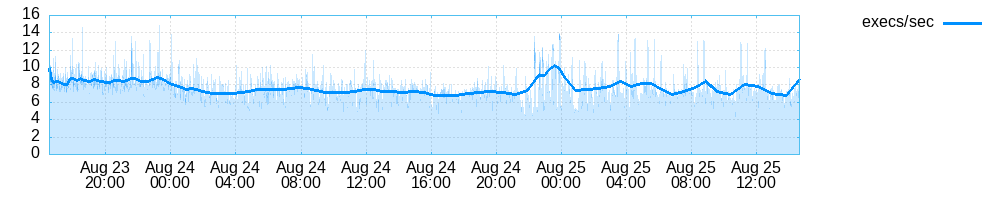
\includegraphics[width=\textwidth]{img/exec_speed}
    \caption[Diagramm zur Veranschaulichung der Ausführungsgeschwindigkeit von AFLNet während der Fuzzing-Kampagne]{Diese Abbildung zeigt die Ausführgeschwindigkeit von \gls{afl}Net.
    Es wird die Anzahl der Nachrichtensequenzen pro Sekunde (y-Achse), die an das \gls{zup} während des Zeitrahmens der
    Kampagne (x-Achse) gesendet wurden, veranschaulicht.}
    \label{fig:aflnet_execs}
\end{figure}
\noindent Die Ausführungsrate ist eine Metrik, um den Fortschritt und die Effektivität einer Fuzzing-Kampagne zu bewerten.
Eine hohe und stabile Ausführungsrate deutet auf einen effizienten Fuzzing-Prozess hin, während Schwankungen oder ein
Rückgang auf potenzielle Engpässe oder Herausforderungen während der Kampagne hinweisen können.\newline
Die Ausführungsrate liegt im Durchschnitt zwischen 6 und 10 execs/sec und zeigt eine gewisse Variabilität, wie durch die
Spitzen und Täler in der hellblauen Schattierung dargestellt.
Anzumerken ist, dass das \gls{zup} mit einem AddressSanitizer kompiliert wurde, was die Ausführungsgeschwindigkeit
beim Fuzzing verlangsamt.
Das resultiert aus dem zusätzlichen Speicher, welchen bei Start des Programms allokiert wird, um die Speicherzugriffe
zu überwachen.
Zu Beginn der Kampagne gibt es einen kurzen Zeitraum mit erhöhter Variabilität, bevor sich die Ausführungsrate stabilisiert.
Im weiteren Verlauf der Kampagne ist eine leichte Abnahme der Ausführungsrate zu beobachten, gefolgt von einer leichten
Erholung gegen Ende der Kampagne.
Die Kurve zeigt während der gesamten Kampagne eine relativ konstante Ausführungsrate mit periodischen Schwankungen.
Diese Schwankungen können auf mehrere Faktoren zurückzuführen sein, darunter:
\begin{itemize}
    \item Komplexität der zu testenden Eingaben: Komplexere Testfälle können mehr Zeit in Anspruch nehmen, was die Ausführungsrate verringert.
    \item Systemressourcen: Veränderungen in der Verfügbarkeit von Systemressourcen (z.B.\ CPU, Speicher) können ebenfalls die Ausführungsrate beeinflussen.
    \item Optimierungen oder Veränderungen im Fuzzing-Prozess: Wenn das Fuzzing-Tool neue Pfade oder besonders anspruchsvolle Testfälle entdeckt, kann dies die Rate der durchgeführten Tests vorübergehend senken.
\end{itemize}
\noindent Ein leichtes Absinken der Ausführungsrate zwischen dem 24. August, 12:00 Uhr, und dem 25. August, 00:00 Uhr, ist bemerkenswert.
Dies könnte darauf hindeuten, dass in dieser Phase anspruchsvollere Testfälle bearbeitet wurden oder dass die Systemressourcen
temporär begrenzt waren.
Die anschließende Erholung der Ausführungsrate könnte durch die Verarbeitung weniger komplexer Testfälle oder eine bessere
Ausnutzung der Systemressourcen erklärt werden.
Die insgesamt stabile Ausführungsrate über den Zeitraum von 48 Stunden deutet auf einen stabilen Fuzzing-Prozess hin.
Die beobachteten Schwankungen sind im Rahmen dessen, was bei längeren Fuzzing-Kampagnen zu erwarten ist, und weisen auf
die normale Dynamik im Fuzzing-Prozess hin, wenn unterschiedliche Testfälle mit variierender Komplexität ausgeführt werden.
Die leichte Abnahme der Ausführungsrate gegen Ende der Kampagne könnte als Hinweis darauf gewertet werden, dass das Tool
zunehmend anspruchsvollere Testfälle oder Pfade bearbeitet hat.
Außerdem anzumerken ist, dass eine Ausführung von \gls{afl}Net dem Starten des \gls{zup}, dem anschließenden
Senden einer Nachricht aus dem Fuzzing Corpus und dem Beenden des \gls{zup} entspricht.
Dem zu entnehmen ist, dass bei Komplexen \gls{iot} Protokollen die Ausführungsrate geringer ausfallen kann, da die
Initialisierung des \gls{zup} und das Senden einer Nachricht mehr Zeit in Anspruch nehmen kann.
\begin{figure}[H]
    \centering
    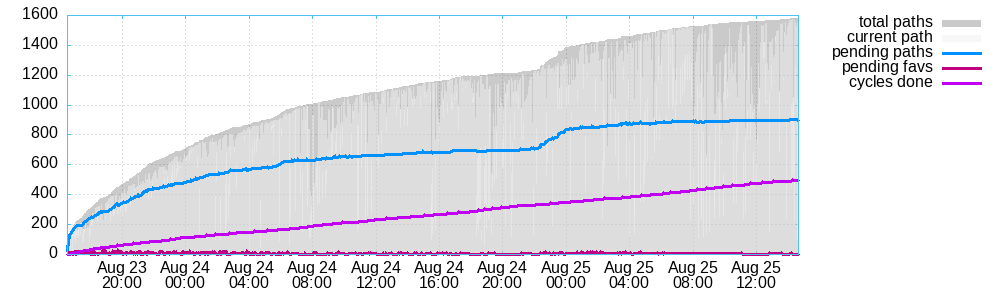
\includegraphics[width=\textwidth]{img/high_freq}
    \caption[]{Das Diagramm veranschaulicht das Eingabegenerierungsverhalten von \gls{afl}Net während der Fuzzing-Kampagne.
    Die y-Achse gibt einen numerischen Wert an, welcher im Kontext zu den abgebildeten Graphen zu betrachten ist.}
    \label{fig:aflnet_speed}
\end{figure}
\noindent Das gezeigte Diagramm veranschaulicht den Verlauf einer 48-stündigen Fuzzing-Kampagne mit dem \gls{afl}Net-Tool, wobei
verschiedene Metriken im Zusammenhang mit der Testabdeckung und dem Fortschritt des Fuzzing-Prozesses dargestellt werden.
Im Folgenden werden die verschiedenen Kurven analysiert und ihre Bedeutung in Bezug auf die Kampagne erläutert.\newline\newline
Die graue Fläche (siehe Abb.~\ref{fig:aflnet_speed}) zeigt die Gesamtanzahl der explorierten Pfade während der Kampagne.
Diese Zahl steigt kontinuierlich an und erreicht gegen Ende der Kampagne über 1400 Pfade.
Der gleichmäßige Anstieg deutet darauf hin, dass der Fuzzer während der gesamten Kampagne effektiv neue Pfade
identifizieren konnte.
Interessanterweise gibt es Phasen, in denen der Anstieg steiler ist, was auf eine besonders hohe Entdeckungsrate neuer
Pfade in diesen Perioden hinweist.\newline
Die hellblaue Linie (siehe Abb.~\ref{fig:aflnet_speed}) repräsentiert den aktuell im Test befindlichen Pfad.
Diese Kurve zeigt, wie das Fuzzing-Tool ständig neue Pfade auswählt und testet.
Die Linie verläuft relativ flach, was darauf hinweist, dass das Fuzzing-Tool regelmäßig zwischen den Pfaden wechselt und
keiner besonders lange untersucht wird.
Diese regelmäßige Bewegung zwischen den Pfaden kann auf eine gleichmäßige Verteilung der Testressourcen hinweisen.\newline
Die Anzahl der noch zu testenden Pfade (blau, siehe Abb.~\ref{fig:aflnet_speed}) zeigt einen Anstieg, der während der gesamten Kampagne
andauert und gegen Ende der 48 Stunden fast 600 erreicht.
Dies bedeutet, dass das Fuzzing-Tool konstant neue Pfade entdeckt hat, die es noch zu testen gilt.
Der kontinuierliche Anstieg zeigt, dass das System immer neue potenziell interessante Zustände produziert, die eine
weitere Untersuchung erfordern.\newline
Die lila Kurve (siehe Abb.~\ref{fig:aflnet_speed}) stellt die favorisierten Pfade dar, die noch nicht getestet wurden.
Diese Zahl steigt ebenfalls stetig an, jedoch langsamer als die \enquote{pending paths}(siehe Abb.~\ref{fig:aflnet_speed}).
Dies deutet darauf hin, dass das Fuzzing-Tool bestimmte Pfade als besonders wichtig erachtet und diese bevorzugt behandelt,
obwohl noch viele andere Pfade auf ihre Untersuchung warten.
Diese Priorisierung kann dazu beitragen, dass besonders interessante oder sicherheitsrelevante Pfade frühzeitig getestet werden.
Die magentafarbene Kurve (siehe Abb.~\ref{fig:aflnet_speed}) zeigt die Anzahl der abgeschlossenen Testzyklen.
Diese steigt über die Zeit an, was die Fortschritte im Fuzzing-Prozess darstellt.
Ein Zyklus umfasst die vollständige Durcharbeitung des aktuellen Satzes von Testfällen.
Der Anstieg zeigt, dass das Fuzzing-Tool kontinuierlich neue Zyklen durchläuft, was auf eine fortlaufende und systematische
Prüfung der Pfade hinweist.
\begin{figure}[H]
    \centering
    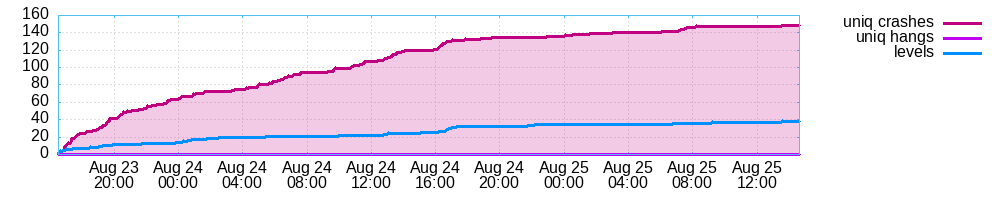
\includegraphics[width=\textwidth]{img/low_freq}
    \caption[Grafik zur Veranschaulichung der Gefundenen Bugs mit AFLNet]{Diese Abbildung zeigt die Anzahl der gefundenen
    Bugs (auf der y-Achse) von \gls{afl}Net in Relation zur vergangenen Zeit (x-Achse).}
    \label{fig:aflnet_bugs}
\end{figure}
\noindent Die Anzahl der einzigartigen Abstürze (pink siehe Abb.~\ref{fig:aflnet_bugs}) zeigt einen kontinuierlichen Anstieg über den gesamten Kampagnenzeitraum.
Besonders auffällig ist der steile Anstieg zu Beginn der Kampagne, gefolgt von einem moderateren Anstieg, der sich über
den Rest der Kampagne hinweg fortsetzt.
Dies deutet darauf hin, dass in den ersten Stunden der Kampagne eine größere Anzahl an Abstürzen entdeckt wurde, was
typisch für Fuzzing-Kampagnen ist, bei denen anfänglich viele triviale Schwachstellen gefunden werden.
Im weiteren Verlauf der Kampagne werden dann weniger neue Abstürze entdeckt, was darauf hinweist, dass das System bereits
viele der simpleren potenziellen Schwachstellen aufgedeckt hat.
Die Anzahl der einzigartigen Hänger (magenta, siehe Abb.~\ref{fig:aflnet_bugs}) bleibt über den gesamten Kampagnenzeitraum stabil bei null.
Dies könnte darauf hindeuten, dass entweder keine Hänger im getesteten System aufgetreten sind oder dass das verwendete
Fuzzing-Setup nicht in der Lage war, solche Zustände effektiv zu identifizieren.
Die Levels-Kurve (blau, siehe Abb.~\ref{fig:aflnet_bugs}) zeigt nur einen leichten Anstieg in den ersten Stunden der Kampagne und bleibt danach weitgehend konstant.
Dies könnte darauf hinweisen, dass nur wenige neue Code-Pfade (Levels) während des Fuzzings entdeckt wurden, was
möglicherweise auf die Komplexität des Zielsystems oder auf die Grenzen der verwendeten Mutationsstrategien hinweist.
Die Fuzzing-Kampagne mit \gls{afl}Net war erfolgreich darin, eine beträchtliche Anzahl einzigartiger Abstürze zu entdecken,
insbesondere in den ersten Stunden des Fuzzings.
Der Mangel an identifizierten Hängern und der begrenzte Anstieg an Levels könnte jedoch darauf hinweisen, dass entweder
das Zielsystem keine anfälligen Hängerzustände aufweist oder dass das Fuzzing-Setup verbessert werden könnte, um diese
Art von Fehlern besser zu identifizieren.
\subsubsection{Analyse der gefundenen Bugs}\label{subsubsec:bugs}
Die gefundenen Bugs nach der 48-stündigen Fuzzing-Kampagne belaufen sich auf 151 Bugs (siehe Abb.~\ref{fig:aflnet_bugs}).
Hierzu wurden alle Abstürze mithilfe von Bash-Skripts dokumentiert~\cite{crash-extraction-script} und analysiert~\cite{analyse-crashes-script}.
Bei allen gefundenen Bugs handelt es sich um \textit{Segmentation Faults} und konnten in vier Kategorien eingeteilt werden:
\begin{enumerate}
    \item Absturz durch Buffer Overflow in der Funktion \texttt{packet\_\_write\_bytes} \\in \texttt{lib\/packet\_datatypes.c}
    \item Absturz durch Buffer Overflow in der Funktion \texttt{packet\_\_write\_bytes} \\in \texttt{lib\/packet\_datatypes.c}
    mit einer \gls{qos}-Nachricht
    \item Absturz durch Buffer Overflow in der Funktion \texttt{packet\_\_write\_bytes} \\in \texttt{lib\/packet\_datatypes.c}
    mit einer \gls{qos}-Nachricht und einem subscriber
    \item Absturz durch Buffer Overflow in der Funktion \texttt{handle\_\_publish} in \\\texttt{src\/handle\_publish.c}
\end{enumerate}
Die Abstürze der vierten Kategorie sind auf die eigene Implementierung eines Buffer Overflows zurückzuführen.
Dieser Buffer Overflow wird getriggert, da die Sanity-Checks (~\ref{lst:mqtt-sainity-checks}) in der Funktion \texttt{handle\_\_publish} auskommentiert
wurden.
Diese Sanity-Checks überprüfen, ob die Länge der Nachricht, die an den Broker gesendet wird, korrekt ist.
Der Fehler tritt nach dem auskommentierten Sanity-Check auf, wenn darauf geprüft wird, ob die Nachricht, die gesendet
werden soll bereits existiert.
Hierzu soll die gesendete Nachricht -- mit einer bereits vorhandenen Nachricht-ID -- mit der bereits zwischengespeicherten
Nachricht verglichen werden.
Diese Nachricht mit der gleichen ID ist jedoch größer als die bereits zwischengespeicherte Nachricht und führt bei dem
Vergleich mit \texttt{memcmp} zum Absturz des \gls{zup}.
\newline
Die anderen drei Kategorien sind gleichen Ursprungs.
Hier handelt es sich um einen Buffer Overflow in der Funktion \texttt{packet\_\_write\_bytes} in der Datei \\
\texttt{lib\/packet\_datatypes.c}.
Diese Schwachstelle wird bei dem Senden der Nachricht an ein Topic ausgelöst.
Hierbei werden Nachrichten vom Broker empfangen und das Topic weitergeleitet.
Wenn Subscriber auf das Topic warten, wird die Nachricht an die Subscriber mittels des Syscalls \texttt{memcpy} weitergeleitet.
\newline
Die Gesamterscheinungen der Bugs belaufen sich auf 151 Bugs, von denen 105 dem Fehler in der Funktion
\texttt{handle\_\_publish} entsprechen.
Die restlichen 46 Bugs entstammen den Buffer Overflows in der Funktion \texttt{packet\_\_write\_bytes}.
\newline
Die gefundenen Bugs wurden mithilfe des Tools \texttt{aflnet-replay} reproduziert und auf ihre Validität überprüft.
Sie zeigten jedoch keine Wirkung auf den Broker ohne manuell implementierte Schwachstellen.\newline\newline
Zusammenfassend lässt sich sagen, dass \gls{afl}Net nur zwei Schwachstellen im Broker Mosquitto gefunden hat, von denen
beide von der Implementierung der Sanity-Checks abhängen.
Wichtig anzumerken ist, dass \gls{afl}Net einen Absturz genau dann als einzigartig betrachtet, wenn die an das \gls{zup}
übergebene Nachricht einen neuen Pfad im Code des \gls{zup} erreicht.
Die Stelle, an der das \gls{zup} zum Absturz gebracht wird, ist für \gls{afl}Net nicht ausschlaggebend.